\documentclass[a4paper]{jpconf}
\usepackage{graphicx}
\usepackage{hyperref}
\usepackage{listings}
\usepackage{color}
\usepackage{enumitem}
%\lstloadlanguages{javascript,xml}
%\pagenumbering{roman}

\definecolor{gray}{rgb}{0.4,0.4,0.4}
\definecolor{darkblue}{rgb}{0.0,0.0,0.6}
\definecolor{cyan}{rgb}{0.0,0.6,0.6}

\lstset{
  language = XML,
  basicstyle=\ttfamily,
  columns=fullflexible,
  showstringspaces=false,
  commentstyle=\color{gray}\upshape
}

\lstdefinelanguage{XML}
{
  morestring=[b]",
  morestring=[s]{>}{<},
  morecomment=[s]{<?}{?>},
  stringstyle=\color{black},
  identifierstyle=\color{darkblue},
  keywordstyle=\color{cyan},
  morekeywords={xmlns,version,type}% list your attributes here
}

\lstset { %
    language=C++,
  %  backgroundcolor=\color{black!5}, % set backgroundcolor
    basicstyle=\footnotesize% basic font setting
}

%
\lstdefinelanguage{JavaScript}{
  keywords={typeof, new, true, false, catch, function, return, null, catch, switch, var, if, in, while, do, else, case, break},
  keywordstyle=\color{blue}\bfseries,
  ndkeywords={class, export, boolean, throw, implements, import, this},
  ndkeywordstyle=\color{black}\bfseries,
  identifierstyle=\color{black},
  sensitive=false,
  comment=[l]{//},
  morecomment=[s]{/*}{*/},
  commentstyle=\color{green}\ttfamily,
  stringstyle=\color{red}\ttfamily,
  morestring=[b]',
  morestring=[b]"
}

\lstset{
   language=JavaScript,
  % backgroundcolor=\color{lightgray},
   extendedchars=true,
   basicstyle=\footnotesize\ttfamily,
   showstringspaces=false,
   showspaces=false,
   numbers=left,
   numberstyle=\footnotesize,
   numbersep=9pt,
   tabsize=2,
   breaklines=true,
   showtabs=false,
   captionpos=b
}

\begin{document}
 % \title{Preparing a paper using \LaTeXe\ for publication in \jpcs}
\title{New ROOT graphics language}

\author{Iliana Betsou, Serguei Linev, Bertrand Bellenot, Olivier Couet}

\address{Production Editor, \jpcs, \iopp, Dirac House, Temple Back, Bristol BS1~6BE, UK}

\ead{iliana.betsou@cern.ch, s.linev@gsi.de, bertrand.bellenot@cern.ch, olivier.couet@cern.ch}

\begin{abstract}
In the context of ROOT7, the graphics system is completely redefined. Based on client
server architecture and with the use of modern C++ and JavaScript, ROOT7 provides a
new web based graphics system. The new concepts of ROOT7 can be displayed directly
in the browsers using the new classes for opening a new web window, communicate
with the server and exchange data between front and back end and JavaScript ROOT (JSROOT).
\end{abstract}

\section{Introduction}
\href{https://root.cern.ch/}{ROOT}~\cite{root} exists for more than two decades and
from the beginning, it has its own graphics system. This graphics system~\cite{Antcheva:2011zz}
used the most popular technologies at that time, like OpenGL and X11. With the rapid development
of technology of the last years and the high turn on the web technology, it was time for
changing the whole graphics system. The new ROOT7's graphics library in ROOT, with the
use of modern C++ and web based architecture, redefine completely ROOT graphics (Figure 1)
 and introduce a new web based environment.
\\
% \begin{figure}[h]
% \includegraphics[width=26pc]{WebEve1.eps}\hspace{2pc}%
% \begin{minipage}[b]{14pc}\caption{\label{label}The new version of web Event Visualization Environment (EVE)}
% \end{minipage}
% \end{figure}
\begin{figure}[h]
  \begin{center}
    \includegraphics[width=15pc]{alice.eps}\hspace{2pc}%
  \end{center}
\centering
\begin{minipage}[b]{25pc}\caption{\label{label}Tracks and hits combined with ALICE detector}
\end{minipage}
\end{figure}


\section{Objectives of the new version}

The current version of ROOT6~\cite{root6} Graphical User Interface (GUI) is very ``OS-specific'' and originally based on X11.
Meanwhile there are different problems, including missing support of X11 on MacOS ~\cite{x11} or difficulties to use OpenGL through remote X11.
Another limiting factor of the current implementation is the missing support of multi-threading. 

To resolve these issues and increase maintainability, new widely used web technologies can be used. This would help to increase portability, 
provides support of remote displays, will enable any future platforms. And by new design multithreading can be provided.
The answer to all the above can be \href{https://root.cern.ch/root-7}{ROOT7}~\cite{root7} development.

\section{ROOT7}

A web based application (as ROOT7) is a client/server computer application (Figure 2),
where the server is a normal ROOT C++ application and the client runs directly in the browser.
The most important classes on the C++ side are {\it THttpServer}~\cite{http} which is responsible
for the communication between the different parts and TBufferJSON~\cite{buffer}
which is responsible for the I/O. The client side is written in JavaScirpt and uses \href{https://root.cern/js/}{JSROOT}~\cite{jsroot}. 
For the implementation of high-level widgets, the \textit{OpenUI5}~\cite{openui} framework is used facilitating the
\href{https://en.wikipedia.org/wiki/Model%E2%80%93view%E2%80%93controller}{Model-View-Controller(MVC)}~\cite{mvc}
architecture. 

\begin{figure}[h]
  \begin{center}
    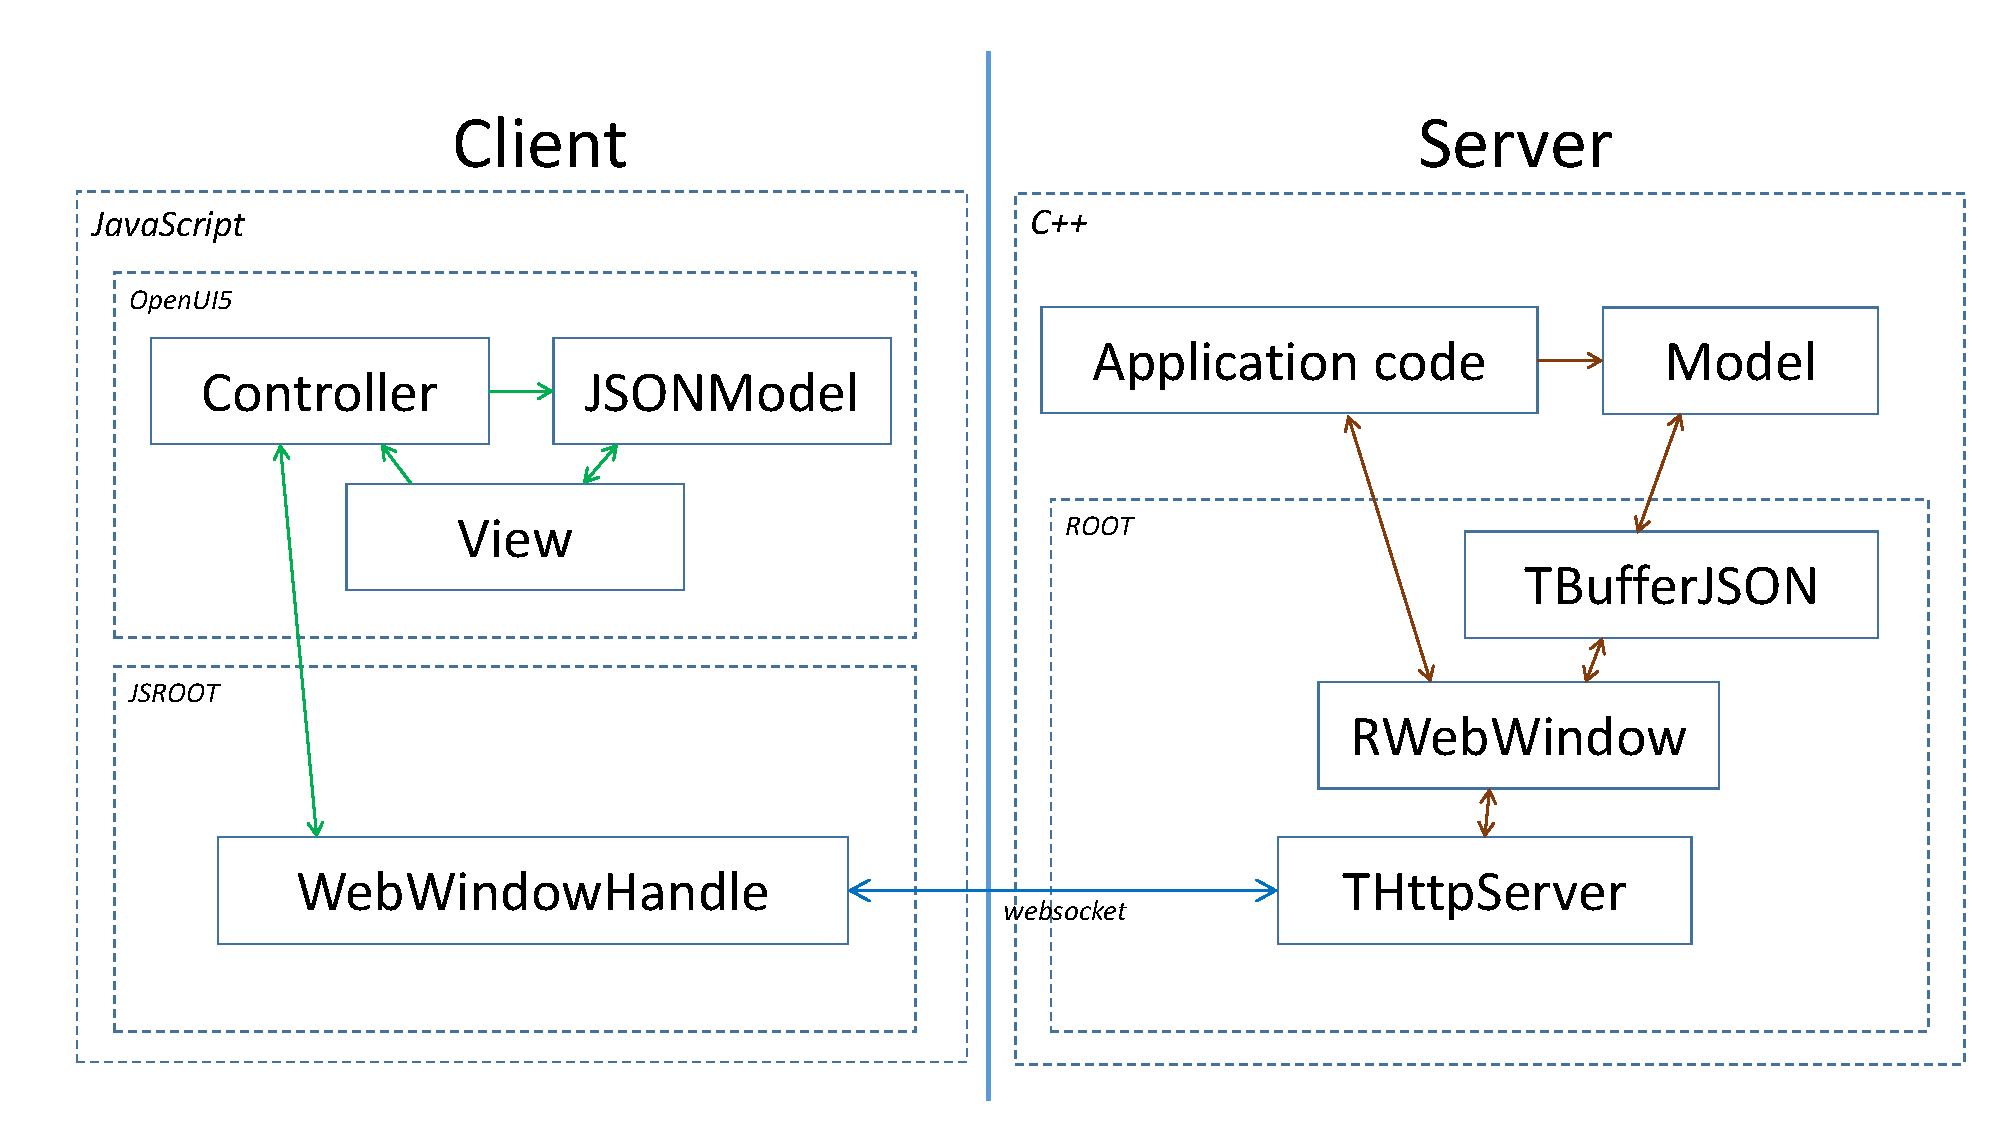
\includegraphics[width=25pc]{figure2.eps}\hspace{2pc}%
  \end{center}
  \centering
\begin{minipage}[b]{20pc}\caption{\label{label}Client Server model}
\end{minipage}
\end{figure}

\subsection{JSROOT}

\href{https://github.com/root-project/jsroot/}{JSROOT} is being developed since
2012 and is responsible for displaying the ROOT objects in web browsers using
JavaScript. The displayed objects can be manipulated directly in
the web browser. JSROOT can read binary data, stored in TFile, including \textit{TTree}.
Also the ROOT JSON format is fully supported. JSROOT is used by the ROOT jupyter interface.

\subsection{THttpServer}

\href{https://github.com/root-project/jsroot/blob/master/docs/HttpServer.md}{{\it THttpServer}} is
one of the most important components~\cite{http}. It gives HTTP access to any running ROOT application
and is responsible for the execution of commands and methods. With {\it THttpServer}
and JSROOT, it is possible to visualize ROOT objects. The communication is achieved
via WebSockets protocol, which is bidirectional and supports binary data. WebSocket
is a communication protocol providing full-duplex communication channels over a
single TCP connection.

\subsection{TBufferJSON}

\href{https://root.cern.ch/doc/master/classTBufferJSON.html}{TBufferJSON} can converts
any streamable C++ object to JSON and vise versa~\cite{buffer}; the custom streamers
can also be supported. With the use of TBufferJSON, the data exchange between the server (C++)
and the client (JavaScript) is simple. The real ROOT I/O remains fully on the server side.

\subsection{OpenUI5}
The design of the GUI layout is based on \textit{\href{https://openui5.hana.ondemand.com/}{OpenUI5}}~\cite{openui}
which is a JavaScript UI library consisting of a really large number of UI controls.
\textit{OpenUI5} implements the MVC~\cite{mvc} architecture, which split
the application logic into three separate parts:
\begin{itemize}
  \item The Model component contains the application's dynamic data.
  \item The View component is the final output that ends up in the user's browser and defines how the application's data should be displayed.
  \item The Controller component receives inputs and contains the logic that updates the model or the view, depending on the inputs.
\end{itemize}

\subsection{RWebWindow Class}
The RWebWindow~\cite{rweb} class is a server-side entity in the new ROOT window management.
It displays windows in the web browser and manages multiple connections with the clients.
This class transfers the data from and to the clients. It also supports the batch
mode (by using \textit{headless} mode).

 \subsection{Graphics Model}
 The new graphics model is independent from any local graphics backend. It allows
 remote display on all kind of devices. The JavaScript rendering is able to be
 performed in a local canvas.

There are three main components in the ROOT7 graphics model:
\begin{enumerate}[label=\alph*)]
  \item The \textit{Pad} is a base entity containing the list of graphics objects to be drawn and is implemented by the \textit{\href{https://root.cern.ch/doc/master/classROOT_1_1Experimental_1_1RPad.html}{RPad}} class.
  \item The \textit{Canvas} is the window's topmost pad, implemented by \textit{\href{https://root.cern.ch/doc/master/classROOT_1_1Experimental_1_1RCanvas.html}{RCanvas}}.
  \item The \textit{Drawable} entity. A drawable can be anything that can be drawn on a pad. Each drawable entity has a \textbf{GetDrawable} method and is implemented in the \textit{\href{https://root.cern.ch/doc/master/classROOT_1_1Experimental_1_1RDrawable.html}{RDrawable}} class.
\end{enumerate}

% \begin{figure}[h]
% 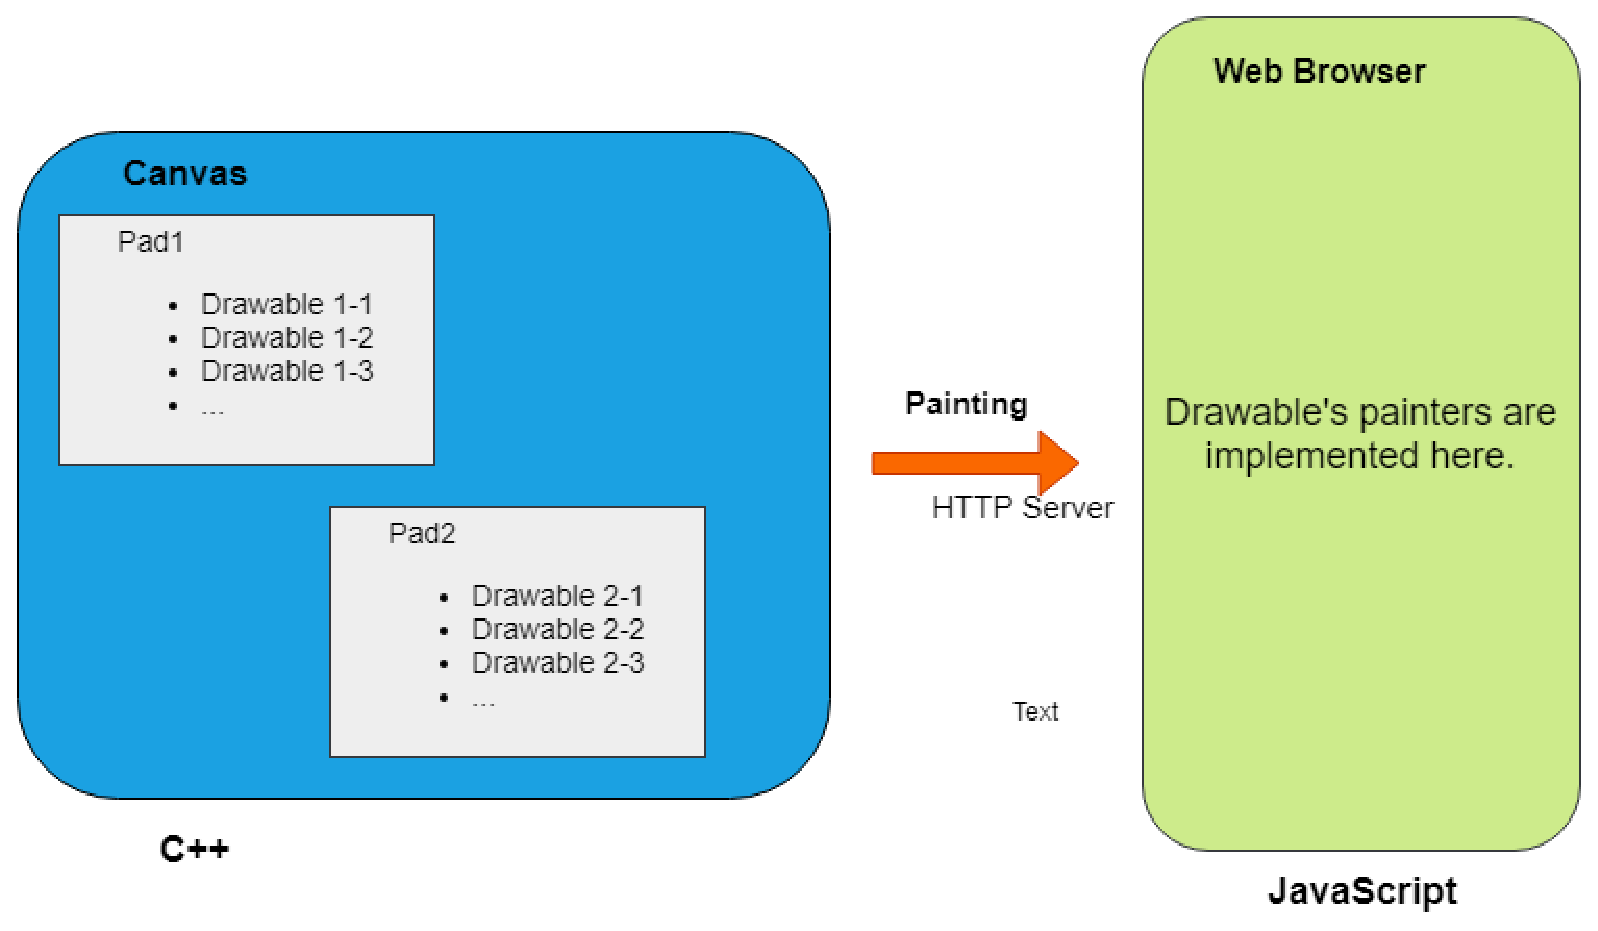
\includegraphics[width=26pc]{BasicConcepts.eps}\hspace{2pc}%
% \begin{minipage}[b]{14pc}\caption{\label{label}Basic Concepts of ROOT7}
% \end{minipage}
% \end{figure}

\subsection{Batch Output}

In the current state of ROOT, there are two main kinds of batch output images:
\begin{itemize}
  \item \textbf{Vector graphics output} (like PDF and SVG) which is implemented by the native ROOT classes
  \item \textbf{Bitmap output} (like PNG and JPEG) which is implemented natively on top of libAfterImage
\end{itemize}

In the new ROOT7, the batch output doesn't rely on any dedicated ROOT graphics
libraries, but it is based on the \textit{}{Headless mode} provided by the web
browsers. In this mode, the graphics is generated in the background by the browser, re-using exactly the same code again and storing result in the output files. 

\section{Example: Fit Panel}

The new version of the \href{https://root.cern.ch/fit-panel}{Fit Panel} is a simple
example of the use of all the above, in particular the \textit{OpenUI5} environment.

The \textit{Fit Panel} is a user interface based on a client/server model and it runs directly
in the browser. The layout is based on the \textit{OpenUI5} framework. It uses all the
power of the ROOT fitting tools to interactively fit histograms, using predefined
functions (such as Gaus, Exponential, Polynomial) or any function defined by
the user. The user is able to choose between several options. There are options
for different ROOT libraries and minimization methods along with a lot of fit
and draw options as well as specific range selector to define the range of the
histogram to be fit. The new and old layout of the \textit{Fit Panel} is shown on Figures 3 and 4.

\begin{figure}[h]
  \centering
\begin{minipage}{14pc}
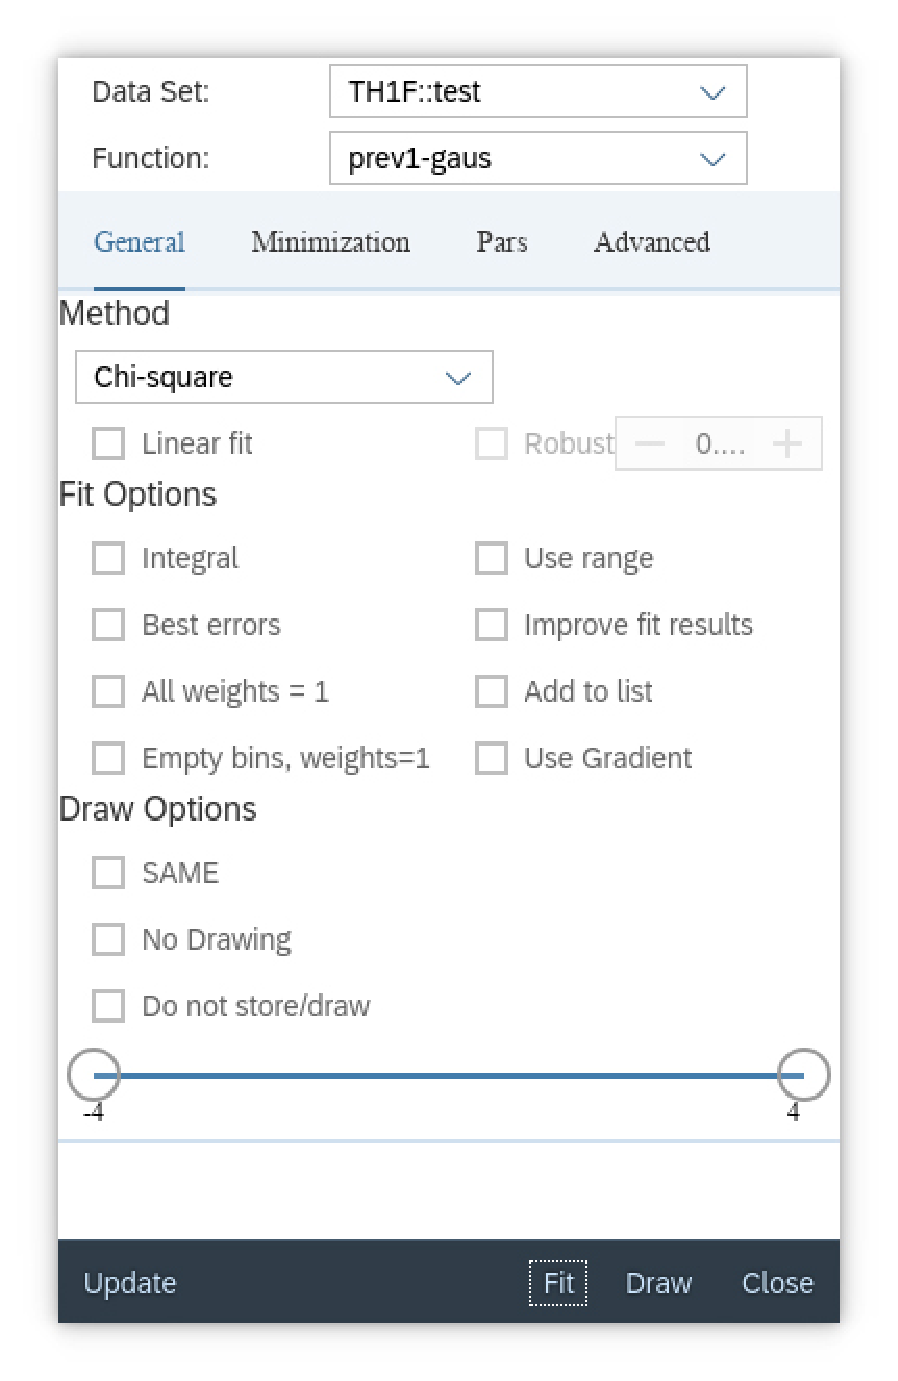
\includegraphics[width=16pc]{rfitpanel1.eps}
\caption{\label{label}ROOT7 version of the Fit Panel}
\end{minipage}\hspace{2pc}%
\begin{minipage}{14pc}
\includegraphics[width=15pc]{oldPanel.eps}
\caption{\label{label}ROOT6 version of the Fit Panel}
\end{minipage}
\end{figure}


The fit Panel includes a lot of different UI controls - text, items lists or selected values provided by ROOT as \textit{JSONModel} class of \textit{OpenUI5}. 
A small but indicative example shows how the \textit{ComboBox} control can be dynamically filled and selection results can be used on the C++ side.

The first step is the creation of C++ structures, which can represent all necessary data for \textit{ComboBox}:

\begin{lstlisting}[language=C++,numbers=none]
     // single item
     struct RComboBoxItem {
        std::string key;
        std::string value;
        RComboBoxItem() = default;
        RComboBoxItem(const std::string &k, const std::string &v) : key(k), value(v) {}
     };
     // complete structure 
     struct RFitPanelModel {
        std::vector<RComboBoxItem> fItems;
        std::string fSelected;
     };
\end{lstlisting}

The model structure includes vector of items \textit{fItems} and selected element \textit{fSelected}.
This structure should be filled with the actual values and send to the client as JSON, using the \textit{TBufferJSON} class for transformation:

\begin{lstlisting}[language=C++,numbers=none]
     RFitPanelModel model;
     model.fItems = {{"id0", "value0"}, {"id1", "value1"}, {"id2", "value2"}};
     model.fSelected = "id1";
     auto json = TBufferJSON::ToJSON(&model);
     fWindow->Send(fConnId, "MODEL:"s + json.Data());
\end{lstlisting}

Produced JSON code:

\begin{lstlisting}[language=JavaScript,numbers=none]
      {
        "_typename" : "RFitPanelModel",
        "fItems" : [{
          "_typename" : "RComboBoxItem",
          "key" : "id0",
          "value" : "value0"
        }, {
          "_typename" : "RComboBoxItem",
          "key" : "id1",
          "value" : "value1"
        }, {
          "_typename" : "RComboBoxItem",
          "key" : "id2",
          "value" : "value2"
        }],
        "fSelected" : "id1"
      }
\end{lstlisting}

When such data is received by the JavaScript client, it should be parsed and the model object assigned to the view:

\begin{lstlisting}[language=JavaScript,numbers=none]
    if (msg.find("MODEL:") == 0) {
       obj = JSROOT.parse(msg.substr(6));
       this.getView().setModel(new JSONModel(obj));
    }
\end{lstlisting}

For displaying the \textit{ComboBox} with provided data, it should be defined in the XML view file as follow:

\begin{lstlisting}[language=XML,numbers=none]
      <ComboBox 
         selectedKey="{/fSelected}"
         items="{ path: '/fItems' }">
            <core:Item key="{id}" text="{text}"/>
      </ComboBox>
\end{lstlisting}

And the produced \textit{ComboBox} element can be seen in Figure 5.

\begin{figure}[h]
  \begin{center}
    \includegraphics[width=10pc]{testCombo.eps}\hspace{2pc}%
  \end{center}
  \centering
\begin{minipage}[b]{20pc}\caption{\label{label}The produced \textit{ComboBox}}
\end{minipage}
\end{figure}

Once an option is selected, it should be send back to the server side in JSON format.

\begin{lstlisting}[language=JavaScript,numbers=none]
     var json = this.getView().getModel().getJSON();

     this.websocket.Send("MODEL:" + json);
\end{lstlisting}

The final step is decoding such JSON data in C++ and processing corresponding ROOT functions:

\begin{lstlisting}[language=C++,numbers=none]
    if (str.find("MODEL:") == 0) {
       std::string json = str.substr(6);

       auto model = TBufferJSON::FromJSON<RFitPanelModel>(json);

       if (!model) {
          // failure in JSON decoding, handle
       } else if (model->fSelected == "id0") {
          // do first branch
       } else if (model->fSelected == "id1") {
          // do second branch
       } else if (model->fSelected == "id2") {
          // do third branch
       }
    }
\end{lstlisting}

This simple example shows how the \textit{ComboBox} control of \textit{OpenUI5} can be used for item selection from a provided list.
The correspondent structure for the Fit Panel is much more complex, but follows exactly the same logic. 
The main advantage of such approach - exactly the same data structures are used for communication in both directions.


\section{Conclusion}

As the current graphics standards are slowly vanishing, the ROOT framework should
base its graphics and GUI on the technologies of the next decades. ROOT7 proposes
this new modern approach by being fully web oriented and based on de facto standards
like SVG or WebGL. Being based on a client/server model, it also allows to completely
discouple the data from its graphics representation. In the same way the GUI tools
are also acting on the data, and they are not embedded in the main application.
The batch output remains an issue but the browsers' headless mode provides an elegant solution.


\section{References}
\bibliography{iopart-num}
\end{document}
